\documentclass[letterpaper,twocolumn,10pt]{article}
\usepackage{usenix}
\usepackage{endnotes}
\usepackage[tight]{subfigure}
\usepackage{natbib}
\setlength{\bibsep}{0.0pt}

\usepackage{url}
\usepackage{multirow}
\usepackage{array}
\usepackage{epsfig}
\usepackage{footnote}
\usepackage{amsmath}
\widowpenalty=10000
\clubpenalty=10000
\setlength{\parskip}{0pt}
\setlength{\dbltextfloatsep}{.2cm}
\setlength{\dblfloatsep}{.2cm}
\setlength{\textfloatsep}{.2cm}
\setlength{\floatsep}{.2cm}
\setlength{\topsep}{.2cm}
\setlength{\intextsep}{.2cm}
\setlength{\belowcaptionskip}{.2cm}

\begin{document}

\title{\Large \bf On the Design and Implementation of Structured P2P VPNs}

\author{
David Isaac Wolinsky$^{\ast}$,
Linton Abraham$^{\bullet}$,
Kyungyong Lee$^{\ast}$,
Yonggang Liu$^{\ast}$,
\\
Jiangyan Xu$^{\ast}$,
P. Oscar Boykin$^{\ast}$,
Renato Figueiredo$^{\ast}$
\\
$^{\ast}$University of Florida, 
$^{\bullet}$Clemson University
\\
}

\maketitle

%\thispagestyle{empty}

\subsection*{Abstract}
%\begin{sloppypar}
Centralized Virtual Private Networks (VPNs) when used in distributed systems
have performance constraints as all traffic must traverse through a central server.
In recent years, there has been a paradigm shift towards the use of P2P for
VPNs that alleviates the pressure placed upon a central server by allowing
participants to communicate directly, relegating the server to handling session
management and acting as a relay when NAT traversal fails.  Approaches to remove
all centralization have turned towards unstructured P2P systems.
These approaches, currently lack the depth in security options provided
by other VPN solutions.  Additionally, the unstructured systems provide relays
when NAT traversal is unsuccessful, but the scalability in current approaches
has not been validated.

In order to deal with these issues in a method that would even be intuitive
to non-expert users , we propose and implement a novel VPN
architecture using a structured P2P system for peer discovery, session
management, NAT traversal, and autonomic relay selection.  We relegate the use
of a central server for certificate management via a partially automated web
interface.  Additionally, we provide a design and implementation of the first
P2P VPN to support full tunneling, whereby all non-P2P based Internet traffic
routes through a trusted third party.

In this paper, we describe the components of our model and evaluate our
reference implementation quantitatively to compare system and networking
overheads of the different VPN technologies focusing on latency, bandwidth,
and memory usage.  We also discuss some of our experiences with developing,
maintaining, and deploying such a system.
%\end{sloppypar}

\section{Introduction}
A Virtual Private Network (VPN) provides the illusion of a Local Area Network
(LAN) spanning over a public wide area network (WAN) infrastructure, guaranteeing
secure and authenticated communication amongst participants.  Common uses of
VPNs include secure access to enterprise network resources from remote/insecure
locations, connecting distributed resources from multiple sites, and
establishing virtual LANs for multiplayer video games over the Internet.  In
the context of this paper, we focus on VPNs that provide connectivity amongst
individual resources, namely, all resources requiring symmetric connectivity will
need to be configured with VPN software.  Our work is significantly different
in scope from approaches that define VPNs ``as the `emulation of a private
Wide Area Network (WAN) facility using IP facilities' (including the public
Internet or private IP backbones).''~\cite{ip_vpns}.  In these VPNs,
large sets of machines are connected to a WAN-like VPN through one or
more virtual routers.

A centralized VPN server can be a single point of failure, can create a
performance bottlenecks, and can compromise end-to-end security.  Several
alternative approaches that address these issues have been conceived: 1)
support for multiple VPN servers for a single VPN~\cite{openvpn}, 2)
decentralized, managed VPNs that do not differentiate between client and server,
3) the use of P2P connections enabling direct communication amongst peers
bypassing the server, relying on the server only for authentication and session
management~\cite{hamachi, wippien}, and 4) the use of unstructured P2P networks
to form decentralized VPNs~\cite{p2pvpn, n2n, tinc}.

Existing centralized VPN approaches suffer from one or more of the
following issues: reliance on a single session or relay server, non-negligible
cost in deploying and maintaining additional session and relay servers,
performance bottlenecks due to relay servers in central systems or in P2P
systems in lieu of NAT traversal.  While P2P VPN approaches handle these
they each introduce one or more of the following issues: discovering a peer
requires broadcasting over the entire overlay, limited options for security and
authorization, lack of information regarding scalability with environments
that include traversable and non-traversable NATs, lack of support for full
tunnel VPN mode.  While decentralized VPN experience a mix of the
issues presented by centralized and P2P VPNs.

The problems we seek to address with our P2P VPN model include:
%\small {
\begin{itemize}
\setlength{\itemsep}{0pt}
\setlength{\parskip}{0pt}
\item reducing the role of centralization for user authentication in a VPN
\item providing intuitive membership management in a VPN
\item supporting full tunneling of Internet traffic in a P2P system
\item handling relay selection in lieu of unsuccessful NAT traversal
\end{itemize}
%}

A brief overview of our solutions to these problems follows and will
be covered in depth in the rest of this paper.  To provide fully decentralized
run-time connectivity and public-key based management of VPN endpoint
membership, we use an automated certificate authority using an intuitive
web based interface using user managed groups.  For handling general trust
concerns in P2P systems, we use the bootstrapping of a private P2P system 
dedicated only for VPN use.  P2P VPNs introduce significantly more complexity when
attempting to do full tunneling since a simple routing table swap as done
in central VPNs will no longer work. Thus, we investigate two different mechanisms for tunneling all
non-P2P-based Internet traffic to our full tunnel gateway(s).  When nodes
cannot directly communicate, they seek to connect to peers that are
physically close to each other and use them to relay communication.

Overall, the main contribution made in this paper is the design and
implementation of a novel structured P2P VPN overlay architecture.  Many of the
individual components of our solution are not novel in themselves, but rather
the integration of these components and their interaction results in a system
that is unique in supporting:
%\small{
\begin{itemize}
\setlength{\itemsep}{0pt}
\setlength{\parskip}{0pt}
\item automated group-based certificate authority
\item easy to use interfaces for managing VPN members and securing VPN tunnels
\item support for full-tunneling through multiple gateways
\item decentralized NAT traversal with autonomous selection of relays for
non-traversable nodes
\item bootstrapping a private P2P VPN system off an existing public P2P system
\end{itemize}
%}

The rest of this paper is organized as follows.  Section~\ref{vpns} gives an overview
of current VPN technologies with emphasis on decentralization and scalability.
Section~\ref{structured_p2p} introduces P2P structures and our previous work IPOP (IP over P2P).
Section~\ref{p2pvpn} describes the contributions of this paper, namely a feature-full
P2P VPN.  In Section~\ref{evaluation}, we discuss our implementation and present evaluation
comparing a VPN models.  Our experience developing, using, and debugging the
system is presented in Section~\ref{experiences}.  In Section~\ref{related_work}, we
compare and contrast our work with related works.  Finally, we give some
concluding remarks in Section~\ref{conclusions}.

\section{Virtual Private Networks}
\label{vpns}
There exist many different flavors of virtual networking.  This paper focuses on
those that are used to create or extend a virtual layer 3 network.  A few
examples of such technologies include Cisco's Systems VPN and AnyConnect VPN
Client~\cite{ciscovpn} as well as OpenVPN~\cite{openvpn}.  In this section, we
begin by going in depth on client configuration of VPNs, then we describe
different VPN server configurations as highlighted in
Table~\ref{tab:vpn_types}, finally concluding the section by presenting
Table~\ref{tab:vpns}, which presents a qualitative overview of production VPNs.

\begin{table}[h]
\setlength{\itemsep}{0pt}
\setlength{\parskip}{0pt}
\centering
\begin{tabular}[c]{|m{2cm}|m{5cm}|} \hline
Type & Description \\ \hline
Centralized & Clients communicate through one or more servers which are statically
configured \\ \hline
Centralized Servers / P2P Clients & Servers provide authentication, session management, and
optionally relay support while peers attempt to communicate directly with each
other, i.e., P2P links \\ \hline
Decentralized Servers and Clients & No distinction between client and servers,
each member in the system authenticates directly with each other, links between
members must be explicitly defined \\ \hline
Unstructured P2P & No distinction between clients and servers, members either know
the entire network or use broadcast to discover routes between each other \\ \hline
Structured P2P & No distinction between clients and servers, members are usually
within $O(\log N)$ hops of each other via a greedy routing algorithm, use 
distributed data store for discovery \\ \hline
\end{tabular}
\caption{VPN Classifications}
\label{tab:vpn_types}
\end{table}

\subsection{Client VPN Configuration}
\label{clientvpn}
In Figure~\ref{fig:vpn}, we abstract the common features of all VPNs with focus
on the client.  The key components of the client are 1) client software that
communicates with the VPN overlay directly and 2) a virtual network (VN)
device.  During initialization VPN software starts by authenticating with an
overlay or VPN agent, then, optionally, it queries the agent for information
about the network such as the network address space, and finally the VN device
is started.

\begin{figure}[h]
\centering
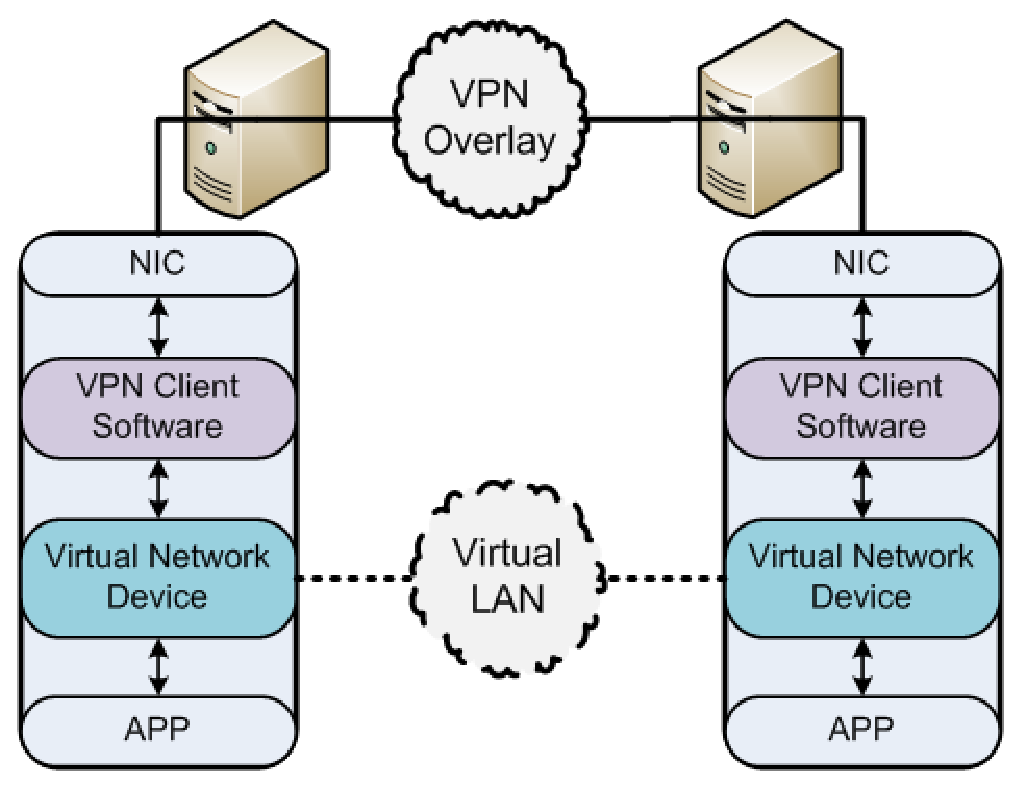
\epsfig{file=figs/vpn.png.eps, width=3in}
\caption{A typical VPN client.  The VPN uses a VN device to make interaction
over the VPN transparent.  Packets that are destined for VPN destinations are
sent via routing rules to the VN device, which acts as like a file descriptor
read and written to by the VPN client.  The VPN client in turn sends and
receives packets over the hosts physical (real) network device.}
\label{fig:vpn}
\end{figure}

There are many different mechanisms for communicating with an overlay agent.
For quick setup, a system may require no authentication or use a shared secret
such as a key or password.  Individual authentication can be provided through the
use of accounts with passwords in addition to a shared secret.  This allows
blocking out users if the shared secret becomes compromised or users act
maliciously.  For the strongest level of security, each client can be
configured to have a signed-certificate that makes brute force attacks very
difficult.  The trade-offs come in terms of usability.  While the use of uniquely
signed-certificates provides better security than shared secrets, it can be more
difficult to set up and use, in particular for a target user base of non-expert.
A good balance found in many environments is the mixture of
a shared secret and individual user accounts, where the shared secret is
included with the installation of the VPN application where the application is
distributed from a secured site.

Once the VPN has connected with the overlay, the VN device
needs to be configured enabling the user's machine to communicate with other
participants in the VPN.  This configuration varies by VPN, commonly though,
this information contains the network address space and an allocation of an
address for the user's machine.

In order to communicate over the VPN transparently, there must exist a network
device driver that allows common network APIs such as Berkeley Sockets and
hence existing application to work without modification.  There are many
different types of VN devices, though due to our focus
on an open platform, we focus on TAP~\cite{tap}. TAP allows the creation of one
or more Virtual Ethernet and / or IP devices and is available for almost all
modern operating systems including Windows, Linux, Mac OS/X, BSD, and Solaris.
A TAP device exists as a block device providing read and write operations. 
Incoming packets from the VN are written to the TAP device and the networking
stack in the OS delivers the packet to the appropriate socket.  Outgoing
packets from local sockets are read from the TAP device.

The VN device can be configured manually through static addressing or
dynamically through dynamic host configuration process (DHCP)~\cite{dhcp0,
dhcp1}.  Once the address to the device is set, a new routing will be added
to the routing table causing all packets sent to the 
VPN address space to be sent to the VN device.  After a packet is read from
the TAP device, it is encrypted and sent to the overlay via the VPN client.
The overlay delivers the packet to another client, which either is a client
or a server enabled with virtual networking stack.  The
received packet is  decrypted, verified for authenticity, and then
written to the TAP device.  In most cases, the IP layer header remains
unchanged while VPN configuration determines how the Ethernet header is handled.

The described configuration so far, creates what is known as a split tunnel,
or a VPN connection that only has passes \emph{VPN related traffic only and
not Internet traffic}.  Another form of tunneling exists called full tunneling.
Full tunneling allows a VPN client to securely forward \emph{all their Internet
traffic} through a VPN router.  This enables a user to ensure all their Internet
communication originates from a secure and trusted location and provides some
level of security when a user is an insecure and potentially hostile
environment, such as an open wireless network at coffee shop.  Both are visually
expressed in Figure~\ref{fig:tunnel}.

\begin{figure}[h]
\centering
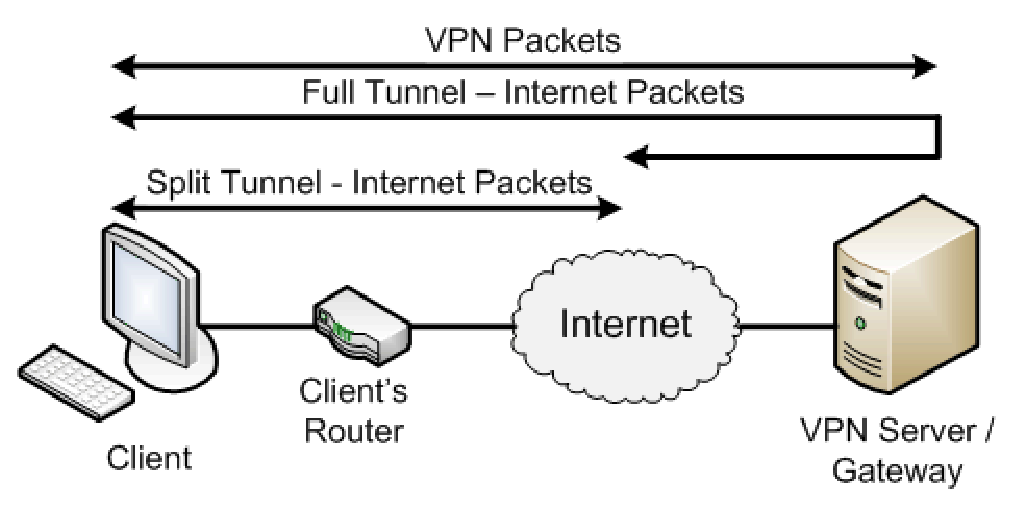
\epsfig{file=figs/tunnel.png.eps, width=3in}
\caption{A VPN setup expressing both full and split tunnel modes.  In both modes,
packets for the server are sent directly to the server.  In split
tunnel mode, Internet packets are routed directly to the Internet.  In full
tunnel mode, Internet packets are first routed to the server / gateway and then
to their Internet destination.}
\label{fig:tunnel}
\end{figure}

Most centralized VPNs implement full tunneling through a routing rule swap,
which makes the default gateway an endpoint in the VPNs subnet and traffic
for the VPN server is routed to the LAN gateway.  As an example, in a 
typical home network, an Internet bound packet will be retrieved at the VN
device, encrypted, and sent to the VPN gateway via the LAN's gateway.  At the
VPN gateway, the packet is decrypted and delivered to the Internet.  All other
traffic is sent to the VN device, then sent securely to the VPN server.  In a P2P
system, there becomes two new considerations 1) P2P traffic must not be routed
to the VPN gateway and 2) there may be more than one VPN gateway.  We further
discuss this issue and provide solutions to this problem in
Section~\ref{fulltunnel}.

\subsection{Centralized VPN Servers}
OpenVPN presents, as its name implies, an open and clear way of implementing a
centralized VPN system.  While there may be minor differences amongst the
different centralized VPN implementations, it is our opinion that OpenVPN
provides a reasonable representation of features found in most centralized VPN.
The key aspects of a centralized VPN server are:

%\small {
\begin{itemize}
\setlength{\itemsep}{0pt}
\setlength{\parskip}{0pt}
\item authentication of clients
\item routing packets between clients
\item providing a NAT to the servers local resources and Internet (full tunnel)
\item inter-server communication
\end{itemize}
%}

Central VPNs server operate at well-known endpoints as in
a universal resource identifier (URI) consisting of a hostname or IP address and
a port.  To log in, clients will randomly attempt to connect to one of the servers until
successful, implementing a simple load balance.  Once connected, clients obtain an
address in the VPN address space.  Depending on configuration this will allow a
client to communicate with other clients, resources on the same network as the
server, or Internet hosts via the VPN.  There are many different ways a
client and server can authenticate with each other.  For a server to authenticate
with a client, the safest way is for the client to have some secure knowledge,
such as the server's certificate, retrieved from a secure source, this can then
be used to verify the server's identity.  The three most common mechanisms for
a client to authenticate with a server are via shared secrets, password, or a
CA-signed certificate.

All client-to-client packets flow through the central server.  In a default
configuration of OpenVPN, the clients encrypt the packet and sends to the server.
The server receives the packet, decrypts it, determines where to relay it, and then
encrypts and sends the packet to the its destination.  This model does not
prevent a server from eavesdropping on client-to-client
communication.  While it is possible, through a shared secret key, that requires
out-of-band communication and is less secure than relying on a CA-signed certificate.

To support full tunneling or allow the client to access the server's resources,
the server too must enable client-like features by becoming a VPN endpoint with
a VN device.  Depending on the configuration, the server can than configure
traffic from the VPN to go through a NAT prior to routing it to the LAN and/or
Internet.  In Section~\ref{fulltunnel}, we present our configuration using
Linux and iptables, a layer 3 network stack manipulator.

OpenVPN allows a distribution of servers, so as to provide fault tolerance and
to a lesser degree load balancing.  Servers must be configured to know about
each other in advance and need routing rules established to forward packets.
Load balancing exists only in the process of the client randomly connecting to
different servers and potentially with a server refusing connection due to load.
There is no distributed load balancing.

%\small{
\begin{table*}[!h!t!]
\setlength{\itemsep}{0pt}
\setlength{\parskip}{0pt}
\centering
%\begin{tabular}[c]{|p{1.1cm}||p{3.475cm}|p{3.475cm}|p{3.475cm}|p{3.475cm}|} \hline
\begin{tabular}[c]{|m{2cm}||m{1.8cm}|m{2.4cm}|m{2cm}|m{2.9cm}|m{3.2cm}|} \hline
& VPN Type & Authentication Method & Peer Discovery & NAT Traversal & Availability \\ \hline \hline

OpenVPN~\cite{openvpn} & Centralized & Certificates or passwords with a central server &
Stored at central server(s) & Relay through server(s) & Open Source\\ \hline

tinc~\cite{tinc} & Decentralized & CA Certificates & Global knowledge &
Relay through mesh & Open Source\\ \hline

CloudVPN~\cite{cloudvpn} & Centralized & CA Certificates & Global knowledge &
Relay through mesh & Open Source\\ \hline

Hamachi~\cite{hamachi} & Centralized P2P & Password at central server & Stored at central server &
NAT traversal and centralized relay & limited free-use, limited Non-Windows
clients, no private relays \\ \hline

GBridge~\cite{gbridge} & Centralized P2P & Password at central server & Stored locally &
NAT traversal, centralized relay & Windows only, freeware, no private relays \\ \hline

Wippien~\cite{wippien} & Centralized P2P & Password at central server & Stored locally & NAT traversal,
no relay support & Mixed Open / Closed source\\ \hline

N2N~\cite{n2n} & Unstructured P2P & Shared secret & Broadcast look up & NAT traversal,
decentralized relay & Open Source \\ \hline

P2PVPN~\cite{p2pvpn} & Unstructured P2P & Shared secret & Global knowledge &
No NAT traversal, decentralized relay & Open Source \\ \hline

IPOP & Structured P2P & CA Certificates or pre-exchanged keys &
DHT look up & NAT traversal and relay through physically close peers &
Open Source\\ \hline

\end{tabular}
\caption{VPN Comparison}
\label{tab:vpns}
\end{table*}
%}

Two examples of systems that assist in distributing load in VPN systems are
tinc~\cite{tinc} and CloudVPN~\cite{cloudvpn}.  Unlike the decentralized P2P
systems, these decentralized systems lack the ability to automatically form
and maintain VPN systems.  In other words, they lack self-organization.  This
means that like OpenVPN, these systems can suffer VPN outages when nodes go offline.
The difference being that OpenVPN makes it explicit who is a server and who
is not, whereas in tinc and CloudVPN anyone can be a server or a client.  In the
typical Tinc and CloudVPN setup, individual users share endpoints with each
other out of band and then place them in the VPN configuration file.  Due to
the lack of self-configuration, members in the system will not replace links
as members go offline.  Thus the mesh, ring, and other structures mentioned
in tinc and CloudVPN documentation require direct human interaction for setup
and management.

\subsection{Centralized P2P VPN Systems}
Hamachi~\cite{hamachi} began the advent of centralized VPNs that went with the
ambiguous moniker ``P2P VPN''.  In reality, these systems would be best
classified as centralized VPNs servers with P2P clients.  Specifically, the
nature of P2P in these~\cite{wippien, gbridge} types of systems provides direct
connectivity between clients once authenticated by a central server.  While
direct connection is desirable, it does not always happen due to firewalls or
impenetrable NATs, when this happens, the central server either acts as a relay
or the two machines are unable to communicate.  One security consideration is
that each of these implementations use their own security protocols that
involve using a server to verify the authenticity and setup secure connections
between clients.  Most of
these projects are closed source, meaning that a user must trust that the
server will not act as a man in the middle and eavesdrop.  Furthermore, these
systems do not support full tunneling nor accessing resources on the same network
as the other client in any of these cases.

\subsection{P2P VPN Client / Server Roles}
\label{introp2p}
Unlike centralized systems, pure (or decentralized) P2P systems have no concept
of dedicated servers, though it is entirely possible to add reliability to the
system by starting dedicated instances of the P2P VPN.  In these systems, all
participants are members of a collective known as an overlay.  Current generation
P2P, decentralized VPNs use a P2P unstructured network, where there are no
guarantees about distance and routability between peers.  Two popular examples of
unstructured P2P VPNs are N2N~\cite{n2n} and P2PVPN\footnote{Due to the similarities
between the name P2PVPN and focus of this paper, P2P VPNs, all occurrences of
the string ``P2PVPN'' refer only to ~\cite{p2pvpn} and all occurrences of P2P VPN refer
explicitly to our research.}~\cite{p2pvpn}.  As a result
participants tend to be connected to a random distribution of peers in the
overlay.  Finding a peer requires either global knowledge of the pool or at
worst case broadcasting a look up message to the entire overlay.  While
unstructured P2P systems have some scalability concerns, P2P systems in general
allow for server-less systems.  In the realm of VPNs, all client VPNs are also
servers with varying different responsibilities depending on the VPN
application, as we present in Table~\ref{tab:vpns}.

Typically, decentralized, P2P VPNs begin by attempting to connect to well-known
endpoints running the P2P overlay software.  A list of such end points can be
easily maintained by occasionally querying the overlay for active participants
on public IP addresses and distributed with the application or some other
out-of-band mechanism.  In the case of P2PVPN, this involves communication with
one or more BitTorrent trackers to find other members of the P2PVPN group. 
N2N~\cite{n2n} requires knowledge of an existing peer in the system.  It uses
this endpoint to bootstrap more connections to other peers in the system,
allowing the application to be an active participant in the overlay and
 potentially be a bootstrap connection for other peers attempting to connect.

\section{Structured Peer-to-Peer Systems}
\label{structured_p2p}
Structured P2P systems provide distributed look up services with guaranteed
search time in $O(\log N)$ to $O(\log_2 N)$ time unlike unstructured systems
that must either know all the state in the system or make random walks
\cite{unstructured_v_structured}.  Some examples of structured systems can be found
in~\cite{pastry, chord, symphony, kademlia, can}.  In general, structured
systems, are able to make these guarantees by self-organization, whereby a node
entering the system follows some form of these abstracted steps:
%\small {
\begin{enumerate}
\setlength{\itemsep}{0pt}
\setlength{\parskip}{0pt}
\item generates or obtains a unique identification number (node ID) on the
order of 128-bits to 160-bits
\item connects to random addresses on a pre-shared well-known endpoints list
\item become connected to at least one peer in the list (leaf connection)
\item look up the peers closest in number to its node ID connecting
to the one immediately smaller and larger than itself (neighbors)
\item connect other nodes in the ring that are further in away in the address
space (shortcuts)
\end{enumerate}
%}

The node ID must be unique to each peer, otherwise there will be an address
collision and the two peers will attempt to connect with the same set of peers.
The peers will only connect to one of them creating disconnectivity.  Furthermore,
having the node IDs well distributed will assist in providing better scalability
as many algorithms for selection of shortcuts depend on having node IDs uniformly
distributed across the entire node ID space.  A simple mechanism to ensure this
is to have each node use a good, cryptographically strong random number
generator.    Applying the birthday problem in this context would require
between $2^{64}$ to $2^{80}$ peers in a system for there to be a 50\% chance of
address collision.  Another mechanism for distributing node IDs involves the use
of a trusted third party to generate node IDs and cryptographically sign
them~\cite{secure_routing}.

Similar to the case of unstructured P2P systems, the incoming node must know
of at least one participant in the system in order to connect to the system.  To
summarize what was stated in Section~\ref{introp2p}, a list of nodes that are
running on public addresses should be maintained and distributed with the
application or be available through some out-of-band mechanism.  Other proposals
suggest using multicast to find pools~\cite{pastry}.  This can work well in
certain environments but multicast range can be quite limited.

Depending on the protocol, a node must be connected to either the closest
neighbor smaller, larger, or both.  Optimizations for fault tolerance suggest
that it should be between 2 to $\log(N)$ on both sides.  If a peer does not
know of the address of its immediate predecessor or successor and a message
is routed through it destined for them, depending on the message type, it may
either be locally consumed or thrown away, never arriving at its appropriate
destination.  Thus having multiple
peers on both sides assist stability when the system is experiencing churn,
especially when peers leave without warning.

Shortcuts make quickly traversing a P2P structure possible.  There are many
implementations and proposals for determining shortcuts, each has differing
costs associated.  A few of these include:  maintaining large tables without
using connections and only verifying usability when routing
messages~\cite{pastry, kademlia}, maintaining a connection with a peer every
set distance from you in the P2P address space~\cite{chord}, or using a handful
of well calculated locations in the node ID space~\cite{symphony}.

\section{Components of a P2P VPN}
\label{p2pvpn}
Before presenting our contributions made in this paper, we first review our
current work as it provides the basis for our P2P VPN.  At the heart of our
system lies a P2P system similar to Symphony~\cite{symphony}, named
Brunet~\cite{brunet}.  The specific components of the system that make it
interesting for use in a P2P VPN system include:
%\small {
\begin{itemize}
\setlength{\itemsep}{0pt}
\setlength{\parskip}{0pt}
\item NAT traversal~\cite{brunet}
\item system stability when two nodes next to each other in address space cannot
directly connect~\cite{hpdc08_0}
\item selection of shortcuts using information based upon proximity~\cite{hpdc08_0}
\item a distributed data store based upon a distributed hash table~\cite{pcgrid07}
\item self-optimizing shortcuts to support single-hop connectivity between peers
in the overlay~\cite{wow}
\end{itemize}
%}

Furthermore, in previous works, we have discussed and implemented a VN with the
following features:
%\small {
\begin{itemize}
\setlength{\itemsep}{0pt}
\setlength{\parskip}{0pt}
\item self-configuring, low overhead use~\cite{sc09, ipop}
\item discovery of members through the use of a virtual DHCP server using
DHT~\cite{sc09, pcgrid07}
\item scalability in the count of hundreds of peers in a single VN~\cite{sc09}
\item portability to any system that supports Tap and Mono\footnote{
Mono is an open source implementation of .Net also known as the Common Language
Run-time (CLR), which provides managed run-time environment similar to Java.}~\cite{mono}
\item ability to behave as a VN interface or router~\cite{sc09}
\item used in grid computing for over 3 years~\cite{archer,vtdc,pcgrid08,gridappliance}
\end{itemize}
%}

Though this framework provides the basis for our design and implementation, we
will attempt to abstract the components as much as possible.

\subsection{Security through Groups}
Setting up, deploying, and then maintaining security can easily become a
non-negligible task.  Most VPN systems that support the use of certificates
require the use of command-line utilities, setting up your own methods of
securely deploying certificates and policing users.  In this section, we
present partially automated certificate management through groups use of a
redistributable web interface.  The key to the group infrastructure is that
users should have a mechanism to verify the authenticity of the server, properly
authenticate themselves with the server, and thereafter acquire signed
certificates as needed.  From an administrators point of view, user information
should be easily available for verification and the ability to ban and remove
users from the pool should be as easy as click a mouse button.

Client usage in our model uses the following process:
%\small {
\begin{enumerate}
\setlength{\itemsep}{0pt}
\setlength{\parskip}{0pt}
\item in a groups environment, a new group is created
\item when a user requests to join, they give relevant information for the group
and agree to some terms of service
\item this triggers an e-mail to be sent to the administrators for the group,
which at a minimum will be the groups creator
\item the administrator can either deny or accept the users access
\item assuming access is provided, the user can then go and download configuration
information
\item this configuration contains the users personal information and a secret
key
\item the user provides the configuration information to the VPN and starts
the service
\item on first boot, the VPN connects with the group web server providing a
certificate request containing the user's node ID and secret key, the server
verifies the authenticity of the user through the secret and ...
\begin{enumerate}
\setlength{\itemsep}{0pt}
\setlength{\parskip}{0pt}
\item automatically signs the certificate
\item or waits for an administrator to verify the certificate request
\end{enumerate}
\item upon receiving a signed certificate, the VPN client connects to the
overlay and can now communicate with other members in the group
\end{enumerate}
%}

Groups provide a decentralized
authentication mechanism and reduce entry barriers into using VPNs.
A group is a trusted set of peers, where the administrator is the
certificate authority signing certificates as he verifies new members and
polices current members.  Signed certificates can be used in decentralized systems as they
do not require communication with the certificate authority, users can verify
that they are members of the group by verifying the signature on the exchanged
certificate.  This removes the need for users to authenticate through a
centralized server and removes the security weakness created by using only user
name and passwords.  An insecure solution for configuration generation would be
to have the server generate a private key and certificate for a peer.  The use
of a binary blob generated by the server allows the user to keep the user's private key
private, but he can also use the blob to generate multiple VPN clients without
direct user interaction from the website.  Securing this system becomes very
important as the blob can easily become a weak spot in the system.  While it may
be cryptographically stronger than a key and password, it must still be
exchanged over secure mediums, such as HTTPS, which can be done with no user
intervention.

Administrators need mechanisms for dealing with malicious users.  In systems
that only use shared secrets, the systems creator has no ability without
collusion to remove malicious participants from the VPN.  Our group model, like
other certificate based schemes, provides the ability to administrate a system
and police such users through the following methods:
%\small {
\begin{enumerate}
\setlength{\itemsep}{0pt}
\setlength{\parskip}{0pt}
\item use a certificate revocation list (CRL) hosted on the web group website
\item sign a revocation and place it into the DHT, peers can verify they are
communicating with trusted peers as often as they like
\item broadcast to the entire P2P system the revocation of the peer
\end{enumerate}
%}

A CRL offers an out of band mechanism for distributing user revocations, unlike
information exchanged in a P2P overlay, primarily because malicious users can
use common P2P attacks to prevent notification of certificate revocations
transmitted via the overlay, but it is significantly more difficult to prevent
the retrieval of a CRL.  Furthermore, if a client is unable to retrieve the
latest CRL, it will be clear that there is a connectivity issue with the CRL
server and it can act appropriately, depending on the security requirements.
The downside is that the CRL is centralized and it can be prohibitively
expensive for peers to verify certificates on regular intervals with short
periods.

The DHT approach allows peers to regularly verify the remote peer prior to
and during connections.  Additionally, DHTs can also be used to implement
event notification, so that the CA can retrieve a list of peers who would like
to be notified if a peer's certificate has been revoked.  The problem with a
DHT is that they can be easily compromised if they have not been implemented
with significant measures to protect against maliciousness.

Finally, the most rudimentary mechanism is broadcasting the certificate
revocation over the entire P2P overlay.  In small networks, the cost of such a
broadcast may be negligible, but as a network grows, such a broadcast may
become prohibitively expensive.  A broadcast can be harder to block through
malicious behavior as a malicious node would need to have significant collusion
in order to completely interrupt the broadcast, though this is feasible in our
model if groups use automated certificate signing.  Furthermore, the broadcast
acts similarly to the DHT event notification, as such, peers find out on a push
like mechanism.  

\subsection{Full-Tunneling over P2P}
\label{fulltunnel}
As discussed in Section~\ref{clientvpn}, VPN tunneling is divided into two
categories:  split tunneling and full tunneling.  In split tunnel mode, the
the VPN client receives and sends messages related only to the VPN, i.e., both
end points are in the VPN; whereas in full tunnel mode, all traffic both VPN
and Internet traffic with the exception of VPN ``control'' messages route over
the VPN, as shown in Figure~\ref{fig:tunnel}.
In a centralized VPN these ``control'' messages would be the
communications directly with the VPN server and full tunnel gateway, which most
likely is the same machine destination IP address from the perspective of the
client.  In a P2P VPN, ``control'' messages would be communications directly
between P2P peers.  Using full-tunneling ensures that a malicious user cannot
easily eavesdrop into what would otherwise be public communication by
forwarding all non-VPN related traffic securely to a third party who resides
in a more trusted environment.  There are two key components to this scheme,
a gateway / server or traffic relayer and a client or a traffic forwarder.
In the following sections, we present a simple scheme for providing gateways
and a few solutions to configuring clients in a structured P2P overlay.

\subsubsection{The Gateway}
Configuring a machine as a gateway can be done with NAT software, in Linux
this is possible through iptables.  One of the components in iptables that
provides NATs is called masquerade, which automatically handles forwarding
packets received on one interface and to the next hop as well as receiving
packets from the Internet and forwarding them back to the appropriate client,
transparently taking care of NAT.  Use of existing NAT software is recommended,
as many applications, including FTP and SIP, embed IP information into the data
of packet, making IP header manipulation insufficient for NAT support.

With a gateway intact, the VPN software can now announce that it provides
full tunneling.  For that purpose, we added an enable flag into the VPN
configuration to specify that a machine is a full tunnel gateway.  When the
VPN software starts, it will automatically append itself to the list of known
gateways for the VPN group in the DHT.

The only remaining difference in VPN gateway is the state machine used in
processing packets coming from the VPN.  Previously, we rejected packets if
the destination was not in the VPN sbunet, now we check first to see if we
have enabled gateway mode.  If it is enabled, all packets are written to the
TAP device with the destination Ethernet address being that of the TAP device.
The remaining configuration is identical to other members of the system.

\subsubsection{The Client}
VPN Clients wishing to use full tunnel must redirect their default traffic to
their VN device.  In our VPN model, we use a ``virtual'' virtual address for
the purpose of providing distributed VN services DHCP and DNS.  This same
address can be used as the VPN gateway, which works fine becase as shown in
Figure~\ref{fig:tunnel_packet}, becase the only sign of that this
packet is destined for the gateway appears at the Ethernet header as the
destination address.  Packets retrieved in the VPN software can then
forward the Internet packet to any machine acting as a gateway without needing
to IP or higher OSI layer changes.  With this in mind, the client software need
only pay heed to the destination IP address, which points to the Internet. 

The VPNs state machine has to be slightly modified to handle outgoing packets
not destined for a remote VPN end point.  If an incoming packet is destined
for some network outside of the VPN address space, full tunnel mode must be
enabled.  If it is enabled, the VPN software will find a remote
peer to act as a full tunnel gateway and then send the packet to the remote peer.

\begin{figure}[h]
\centering
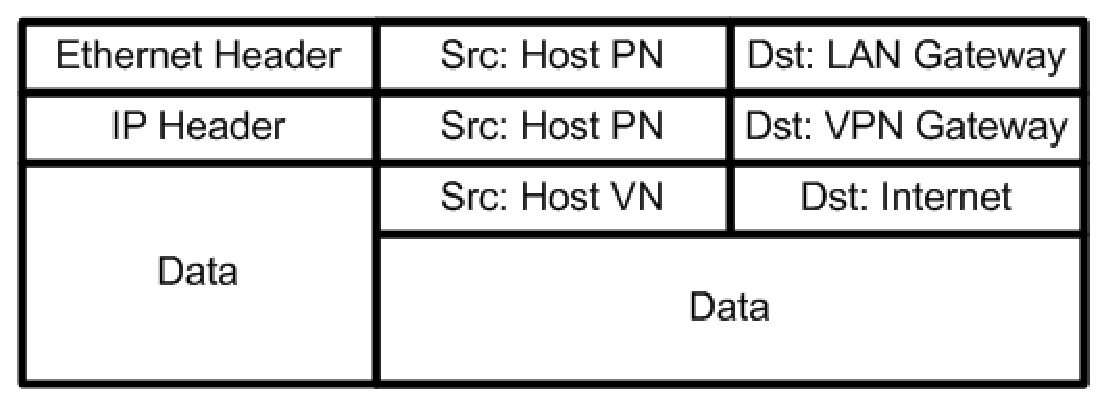
\epsfig{file=figs/tunnel_packet.png.eps, width=3in}
\caption{The contents of a full tunnel Ethernet packet.  PN and VN are defined
as physical and virtual network, respectively.  Interesting components of this
packet are 1) the destination Ethernet address is the LAN gateway, 2) the
destination IP address is the VPN gateway, and 3) the IP payload contains
another IP packet whose source IP is the VN device and destination is the
Internet.}
\label{fig:tunnel_packet}
\end{figure}

The pathway for packets coming back from the Internet will also require some
tweaking, that is, the source IP address will not match the VPN gateways IP.
Thus the VPN client must confirm that the source is a VPN gateway or throw
away the packet.  If the source is authenticated, it can be written to the
VN device and the user application will receive a packet from the Internet.

The two issues in the client configuration are selecting the machine to use as
a gateway and how to ensure P2P packets are sent directly to the remote peer
and not through the gateway.  Our model uses a simple mechanism for determining
which gateway to choose:  query the DHT for a list of potential gateways, select
a random one from the list, and verify liveness via periodic (15 second interval)
ping messages.  For handling faults, we take a pessimistic approach, that is,
if a server is lost, we take note of it and only query the DHT again upon the
next outgoing Internet packet.

For this paper, the second issue, handling P2P routed packets, was the focus of
our work.  Whereas in the centralized VPN case, a client only needs to communicate
directly with a single point in the VPN, which can be done with a single routing
rule change prior to starting the VPN, the same cannot be done for a P2P system.
In a P2P system, ensuring that all P2P overlay messages are routed directly
becomes non-trivial because there will be many such routes most of which will
not be known ahead of time.  If we applied the same model used by centralized VPNs,
the client would end up routing both Internet and P2P traffic through the gateway
machine and if there were disconnection, all state would have to be reinitialized
and more importantly the advantage provided by P2P, scalability, would be lost.
To solve this we present two approaches though in our efforts, we
were only successful with one model for easily setting up a client.  We
present all our work, including our failed attempt, such that it may be the
ground work for further research.

\subsubsection{The Client -- Approach 1 -- Adding Routes}
The first approach taken uses a model similar to the centralized version,
for each P2P machine we communicate with, we add an explicit rule in the
routing table so that packets destined for them are routed directly to them via
the LAN's default gateway.  In order to ensure this, we added a feature to the
socket handling code in our system that would indirectly add the remote nodes
public address to our routing table prior to the first outgoing communication
attempt and would remain in effect until the VPN closed down or the link was no
longer active.  While this model does require unique code for each OS platform,
supporting Linux and Windows was quite trivial.
In this model, Incoming packets will be unaffected by the routing table changes
and will be delivered as they were in the normal system.

This model works well but has two major flaws.  Common to all VPNs that employ
the standard route switch technique, all communication, not just VPN, is routed
directly to the server insecurely.  So while the VPN traffic is most likely
encrypted, if the server also hosts a website, that traffic will be in its natural
state, potentially unencrypted, and visible to any eavesdroppers.  An issue,
unique to our P2P solution, allows a malicious user to send spoofed packets
to have the VPN add extra routes to the routing table, resulting in a similar
situation as the first, unencrypted communication visible to eavesdroppers.
The next two solutions attempted to solve these problems.

\subsubsection{The Client -- Approach 2 -- Ethernet Packets}
This approach recognizes that when using UDP, we know the source port from which
all traffic originates, also even in the case of TCP, we can easily determine
our source ports for outgoing connections using a technique similar to the one
used in the first solution.  While the routing rule directing all traffic to
the VPN remains, there are no additional routing rules.  Thus all packets are
directly sent to the VN device and the VPN client software must handle routing
the packets appropriately.

To distinguish P2P packets from non-P2P packets, the VPN client needs to look
at the source port of outgoing IP packets, if it matches the VPN client's source
port, it must route the packet through the local gateway.  In order to do this,
we need a component that can write to the hosts physical network device an
Ethernet packet to encapsulate the P2P IP packet.  Furthermore, we need to
modify the IP packet to change the source address to match the physical
Ethernet devices IP address.  We focused on two approaches that would be
cross-platform capable: 1) using a bridged tap device whose sole purpose is to
send and receive Internet packets to and from the gateway and 2) using
PCap, a packet capture and injection library, to send packets.  While there
may be other approaches, we focus only on ones that are reasonably portable
to other OSes.

The problem with this approach is that when an incoming packet arrived at the
clients networking stack, the client would not recognize the packet because the
destination IP address was the physical Ethernet's and not the VN Ethernet's,
the one where it originated.  This would trigger the OS either ignoring the
packet in the case of UDP or sending a TCP reset message.  Thus the only
solution would be to implement some form of NAT, that would receive incoming
packets and rewrite them prior to the network stacking thus avoiding a TCP
reset message, a task we have not yet investigated.

\subsection{Autonomic Relays}
A handful of P2P VPNs~\cite{hamachi, gbridge} support relaying when direct
communication is not possible though a majority of them do not.
Centralized and decentralized VPNs do not suffer from this problem
as all traffic passes through the central server or managed links.  Because
of the management and overhead concerns presented by these systems, we propose
the use of distributed, autonomic relaying system based upon previous
work known as ``tunnels''~\cite{hpdc08_0} founded upon principles found in
related work~\cite{epost}.  In this work, we describe a
mechanism using triangle routing that allows peers next to each other in the
node ID space communicate despite them being unable to communicate directly
with each other, whether the cause be firewall, NAT, or Internet
disconnectivity issues.  To support this behavior, two nodes would discover
each other by indirect communication through the overlay.  This would trigger a
best effort to exchange peer lists through the current set of near neighbors.
In most cases, the peers would have at least one overlapping neighbor and the
messages would be exchanged.  Thereafter, peers would use the
overlapping neighbors to communicate with each other ``directly''.

Direct connectivity in most cases provides significant performance gains over
routing through the overlay.  When direct connections is not available, which
is more efficient relaying or overlay routing?  In practical experience, we
have seen overlay transit time in the order of seconds and further establish
the use of relays in our evaluation in Section~\ref{relay_eval}.  When
peers are not near each other in address space, there is a high chance that
they will not have any overlapping peers, thus our current technique would
not work.  Our solution, as represented in Figure~\ref{fig:relay}, is to
have nodes connect to one or more of the remote node's neighbors thus
creating an overlap and our ability to reuse previous work.

\begin{figure}[h]
\centering
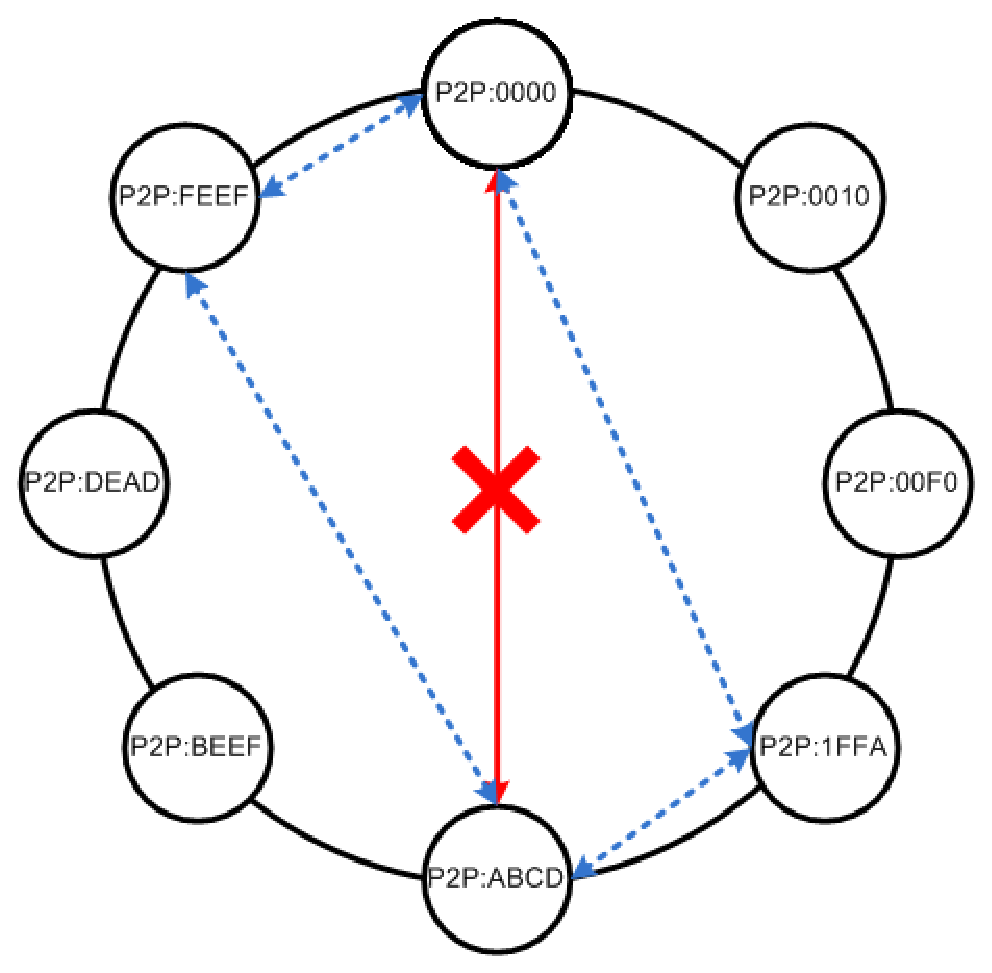
\epsfig{file=figs/relay.png.eps, width=3in}
\caption{Creating relays from across the node address space, when direct
connectivity is not possible.  Two members, 0000 and ABCD,  desire a direct
connection but are unable to directly connect, perhaps due to NATs or firewalls.
They exchange neighbor information through the overlay and connect to one of
each other's neighbors, creating overlap.  The overlap then becomes a a dedicated
relay path (represented by dashed lines), improving performance over relaying
across the entire overlay.}
\label{fig:relay}
\end{figure}

The original approach had one more issue, the lack of consideration
on the viability of relays, the goal was to have connectivity with no
reflection on stability or performance.  To improve this, when exchanging
neighbor lists, we added the ability to exchange arbitrary information
to assist in decision making.  So far we have focused on exchanging connection
stability as measured by the age of the connection between the far node and
his neighbor and the latency between the far node and its neighbor.
Additionally, when overlap changes, we make it optional to select to use
only a subset of the overlap, thus only the fastest or most stable overlap
be used with many more in reserve.  We present our test environment, experiment,
and results.
in~\ref{relay_eval}.

\subsection{Bootstrapping Private Overlays}
In P2P systems, distributed security cannot provide the same level of security
as centralized or managed security.  Hopefully securing an overlay using
well-known security concepts such as PKI and SSL will encourage
wider adoption of P2P systems.  One problem with this approach though is that
users who want a private overlay may not have the resources, i.e. public
addresses, to host there own overlays.  To address this, we suggest
bootstrapping a private overlay from an existing public overlay.  The private
overlay will be completely encrypted and authenticated with only members of the
VPN allowed access.  This work is similar to previous in suggesting the use of
a public overlay to bootstrap application specific overlay has been discussed
in~\cite{one_ring}.

Members of the VPN are the only members of the overlay, providing a powerful
feature that the entire P2P overlay can be secured through groups.  This
prevents malicious users outside of the VPN from attacking it and more easily
enabled the removal of misbehaving peers, primarily rooted in the fact that
the use of a broadcast to signal a certificate revocation is now important to
the entire overlay.

The process for bootstrapping a private overlay follows.  Once the VPN software
begins, it starts by connecting with the public overlay.  It queries the public
overlay's DHT at the key ``private:groupname'', where groupname is the
GroupVPN's name.  The values stored at the key are the public overlay node IDs
of members actively in the private overlay.  The joining VPN software will
attempt to form private overlay leaf (bootstrap) connections with members of this
list over the public overlay.  During this process, both peers verify each
other's authenticity and form a secure connection.  This connection is then used
to bootstrap direct connections with members of the private overlay.  The reason
why the public overlay node IDs are stored at the public overlay's DHT key and
for using private overlay bootstrap connections over the public overlay is to
support NAT traversal.  This model allows reusing Brunets underlying NAT
traversaltechniques to easily bootstrap private overlays.  As a member of a
private overlay, the VPN can somewhat more safely store information in the
private overlay's DHT, relegating the public overlay for private overlay
discovery.  Additionally, the public overlay could be used for relaying, when
direct connectivity is not possible, though this has not been looked into yet.

\section{Evaluation of VPN Models}
\label{evaluation}
For the purpose of quantitatively evaluation, we have added the features of
the proposed design parameters described in Section~\ref{p2pvpn} to IPOP
\cite{sc09} and Brunet~\cite{brunet}.  We present the advantage of using
relays over overlay routing when NAT traversal does not work.  Then we examine
the effects of using different relay selection mechanisms.  Afterwords, we
evaluate the system overheads of OpenVPN, Hamachi, and our P2P VPN to determine
the OS resource costs and the cost of each in a distributed environment.

\subsection{Motivation for Relays in the Overlay}
The purpose of this experiment is to give weight to the argument that relays
are very useful for overlay networks that rely on low latency.  For this
experiment we applied the MIT King data set~\cite{king_data}, a data set
containing all-to-all latencies between 1,740 well-distributed Internet hosts.
We reviewed many different sizes of networks up to 1,740 nodes, evaluating each
network size 100 times.  Our experiments were executed in a simulator, where we
brought the system to steady state.  Once at steady state, we then calculate the average
all-to-all latency for all messages that would have taken two overlay hops
or more, the average of our low latency relay model, and the average of single
hop communication.  In the low latency relay model,
each destination node formia connection to the source nodes physically
closest peer as determined via latency (in a live system by application level
ping).  Then this pathway is used as a two-hop relay between source and node.
We only look at two overlay hops and more as a single hop would not necessarily
benefit from the work and would be the cause of a triangular inequality.

\begin{figure}[h]
\centering
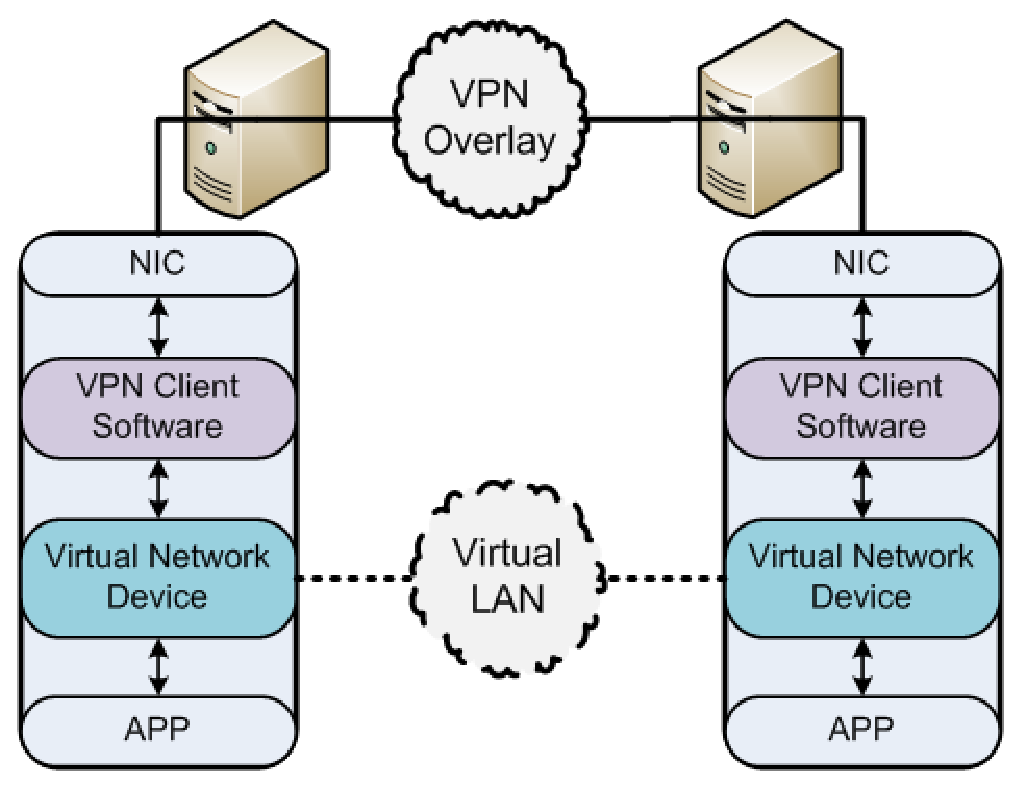
\epsfig{file=figs/vpn.png.eps, width=3in}
\caption{A comparison of the average all-to-all overlay routing, two-hop relay, and
direct connection latency in a Structured P2P environment, Brunet, using the King
data set.}
\label{fig:simulated_relays}
\end{figure}

Our results are presented in Figure~\ref{fig:simulated_relays}.  We performed
the tests for varying network sizes.  In the case of the network size of 10
all peers have direct connections, afterwards, it becomes obvious that the
latency-bound applications using an overlay would significantly benefit from
the use of two-hop relays.  Of course, it goes without saying that a two-hop
relay is not as fast as a direct connection.

\subsection{Comparing Relay Selection}
\label{relay_eval}
In this experiment, we evaluate time to establish a relays and measure bandwidth
and latency provided by the relays.  We perform the experiment on the Hamachi
relay selection as well as our two different models, latency and stability based.  The
setup for the experiment was two VPNs running on the same site but with
firewall, iptables, preventing direct communication.  We then start the VPN and
begin transmitting packets between the peers via Netperf~\cite{netperf}.  We time
how long it takes for a relay to form and then test for latency and bandwidth.
We repeated this test 100 times and present our results in Table~\ref{tab:relay_eval}.
To test latency, we used Netperf in TCP\_RR mode, where it performs a request-reply
between a client and a server.  Bandwidth is determined used Netperf in TCP\_STREAM
mode, which performs a bulk transfer between the client and server.

\begin{table}[h]
\setlength{\itemsep}{0pt}
\setlength{\parskip}{0pt}
\centering
\begin{tabular}[c]{|m{2.2cm}||m{1.3cm}|m{1.3cm}|m{1.4cm}|} \hline
& Setup time (ms) & Latency (ms) & Bandwidth Mbit/s \\ \hline \hline
Hamachi & & & \\ \hline
Latency-aware & & & \\ \hline
Stability-aware & & & \\ \hline
\end{tabular}
\label{tab:relay_eval}
\caption{Results of the Relay evaluation comparing time to establish a relay,
bandwidht, and latency amongst Hamachi's relay service, a latency-focused relay
model, and an stability-focused relay model.}
\end{table}

The results look perculiar, but I can't figure out why.
\subsection{Comparing System Overheads}
In this experiment, we attempt to understand the bounds imposed by OpenVPN,
Hamachi, and IPOP.  We used Amazon EC2~\cite{ec2} to create various sized
networks with various amounts of activity.  The measurements are accumulated
at a single control node as well as the server in the case of OpenVPN.  The
tests begin by doing some initial communication with peers he will communicate
for measurement purposes to warm the system.  Once the system is warmed up,
we continue period pings every 15 seconds for the next 10 minutes.  We
capture the network traffic during this time in bytes and packets transmitted
in to and out of the control and server.  At the end of each test, we
capture total memory currently used by the VPN software.  Tests for the same
network size, begin by communicating with 0 peers and incremently increase
the amount until the control is communicating with all members of the VPN.

\begin{figure}[h]
\centering
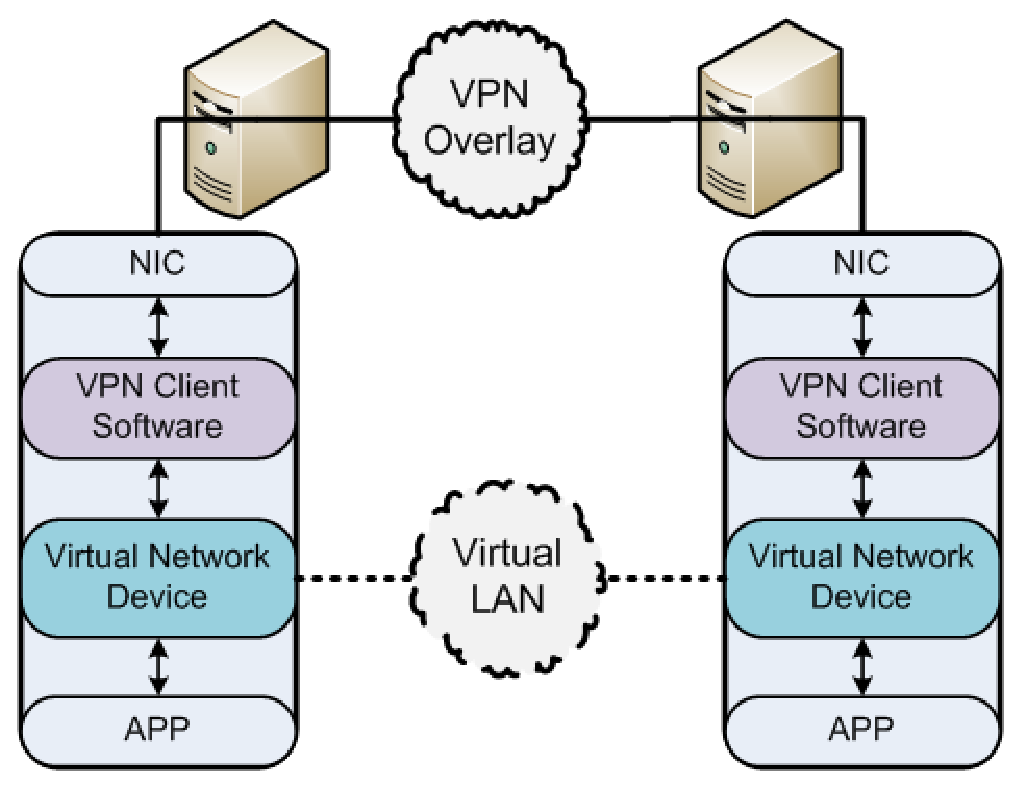
\epsfig{file=figs/vpn.png.eps, width=3in}
\caption{A comparison of the average all-to-all overlay routing, two-hop relay, and
direct connection latency in a Structured P2P environment, Brunet, using the King
data set.}
\label{fig:overheads}
\end{figure}

The results of our test are presented in Figure~\ref{fig:overheads}.

\section{Experiences}
\label{experiences}
Our work on the P2P VPN model presented in this paper is based on four
years of work spent developing, deploying, and maintaining VN software for
grid computing~\cite{wow,vtdc09,archer}.  In this section, we first present
our different deployments involving P2P VPN, then we present our experiences
in debugging a structured P2P system.

\subsection{Deployments}
Initially IPOP was designed to assist in self-configuring adhoc grid deployments
using virtualization.  This can be seen in our project named ``Grid Appliance''
\cite{gridappliance}.  Over the year, the Grid Appliance has matured and so
has our usage of IPOP.  Currently, the Grid Appliance is used as the basis
for a free-to-join computer architecture consisting of over 400 compute resources
spanning 5 seed Universities with users across the United States and the World.
The Grid Appliances allows easy creation of adhoc, distributed grids through
the use of the IPOP and the structured P2P DHT.  Experienced users can use the
system to create large grids in less than an hour with most of the time spent
waiting for virtual machines to boot.  Non-expert users can quickly access the
distributed grid in a matter of minutes by downloading a virtual machine
manager and the Grid Appliance.  The comment we receive most often in our
polls is ``I was surprised at how it just works.''

Motivation for a significant portion of our work lies in our desire to have non-Grid
Appliance connect to Grid Appliances resources in the same ``just works'' manner.
Thus bore our new incarnation of IPOP called GroupVPN, which now is the same
software stack that runs inside Grid Appliance but also allows services the Grid
Appliance to connect with external NFS and external grid resources.

Other work of ours' that relates to IPOP is the SocialVPN~\cite{cops08}.  The
SocialVPN places each client in their own private network, where they are only
addressable by their friends as defined by third party social network.
Unlike GroupVPN, this makes each user the master
of who does and does not have access to their resources.  Though this comes at
the cost of polling a central server, such as Facebook, to determine if a VPN
connection is legitamate, whereas the GroupVPN uses decentralized certificates
signed by a common CA.  SocialVPN does not lend itself well to environments
that require some form of central management such as a computing grid or a
small to medium businesses, for these purposes, we advocate GroupVPN.

\subsection{Discovering Faults}
In literature, the argument typically directed against structured P2P systems
is the ability to handle fault tolerance.  In this section, we share our
tactics for finding faults in a deployed overlay.

Our bootstrap system runs on Planet-Lab~\cite{planetlab}, placing it in that
harsh environment ensures that the system is reliability, stability, and
consistent.  Consistency compares peers knowledge of the pool and tests
each peer for congruence with both its first and second left and right neighbors.
We call this a crawl.  This information is stored in a database, which we can
later use to find nodes that have been inconsistent many consecutive times.
If a node is able to fix inconsistencies in future crawls, experience suggests
the inconsistency was probably due to churn in the system.  Otherwise, it will
probably still be in an inconsistent state and we are able to query the node
and other nodes nearby for state information.  At a minimum, this would be help
us determine if there exists a problem and potentially what state is stale
and causing the connectivity issue.  If this reveals little information, we
either retrieve a log or request it from the user who owns node, the log
typically provides some useful information.  Additionally, as with all
multithreaded applications, deadlocks can happen, we found it useful to add
liveness states to threads to assist in finding deadlocks.

Other information, we watch, includes peer count, memory, and CPU usage.
Node count can be quite difficult to keep track of in Planet-Lab as machines at
a rate of 5 to 20 per day are restarted and our software is not automatically
restarted on these machines, thus the case to watch for is non-linear loss of
nodes.  Planet-Lab also places challenges on memory, as the systems can often be
I/O starved causing what appears to be memory leaks as Brunet's internal queue
can grow without bound.  In these cases, we have the node disconnect from the
overlay and sleep before returning.  The advantage of Planet-Lab as a test ground
is that it presents so many unique situations that can be very difficult to
reproduce in a lab controlled test system.  It is our belief
that any system that uses large scale Planet-Lab deployments as a testing ground
will be quite reliable.

We are still actively seeking better ways to verify the state of our system.
For example, the cost of doing a crawl can take $O(N \log(N))$ time,
since we have to communicate with every single node with an average routing
time of $O(\log(N))$.  For example, current research on Brunet has been focused
on providing a P2P MapReduce~\cite{map_reduce} framework, which can be used to
provide system wide searches and status checks in $O(\log(N))$ time.

\section{Related Works}
\label{related_work}
\subsection{P2P VPN in Other Structured Overlays}
The purpose of this work is to develop a P2P VPN model that can easily be
applied to other structured P2P systems.  In this section, we focus on the
portability of our platform to other structured P2P systems, namely
Pastry and Chord by analyzing FreePastry and
NChord respectively.  FreePastry can easily reuse our C\# implemented
library through the use of IKVM.NET, which allows the porting of
Java code into the CLR.  NChord is a Chord implementation written in C\#.  In
Table~\ref{tab:structured_p2p_compare}, we compare the features of the structured
P2P systems as they apply to the use as a VPN.

\begin{table*}[!h!t]
\setlength{\itemsep}{0pt}
\setlength{\parskip}{0pt}
\centering
\begin{tabular}[c]{|m{2cm}||m{2.75cm}|m{2.8cm}|m{2.95cm}|m{1.65cm}|m{1.65cm}|} \hline
System & Overlay messaging & NAT Traversal & DHT & Secure PtP & Secure EtE\\ \hline
Brunet & Yes (AHSender) & UDP and overlay relaying & Yes with reliability & Yes & Yes \\ \hline
FreePastry & Yes (route) & Only with port-forwarding enabled  & Yes, PAST~\cite{past}, reliable & No & No \\ \hline
NChord & No, only look up & No & Simple, non-fault tolerant DHT & No & No \\ \hline
\end{tabular}
\caption{A comparison of structured P2P systems.  PtP stands for point-to-point
communication, such as communication between physical connections in a P2P
overlay.  EtE stands for end-to-end communication, such as messages routed
over the overlay between two peers.}
\label{tab:structured_p2p_compare}
\end{table*}

The bootstrapping of a connection in NChord, begins by finding the owner of the
DHT key containing the mapping of virtual IP address to node address
through ``find\_successor''.  After establishing a connection, the owner of the
key needs to be queried for the key's value, which would be the node ID of the
node owning the virtual IP.  After executing ``find\_successor'' and retrieving
the destination nodes, the owner of the virtual IPs, physical IP address, the VPN
can ``connect'' to the remote node using either a UDP or TCP socket.  Virtual IP
messages would then be sent and received through this ``connection''.  Unlike
other systems, NChord does not support sending messages through the overlay,
thus a separate ``connection'' for application purposes will need to be
created.

The steps involved in FreePastry begin by looking up the mapping of virtual
IP to node ID in PAST.  The result will be a node ID, which can be called
using ``route'' to send packets and ``deliver'' to handle incoming packets.
In fact, the model is very similar to Brunet.  Furthermore,  FreePastry has
knowledge of proximity in shortcuts, so it may be very easy to apply
high-performance autonomic relays to pastry.  FreePastry does not have
the ability to form shortcuts based upon demands, so if two peers were
actively communicating, they may always have to route traffic over the
overlay, which will probably be significantly slower than if they were
directly connected.  Though one could argue, that since FreePastry does
not support NAT traversal, all nodes will already be public and thus an
application, as in the NChord example, could form a direct connection bypassing
the overlay.

\section{Conclusions}
\label{conclusions}

\bibliographystyle{abbrv}
\small {
\bibliography{nsdi10}
\suppressfloats
}

\end{document}
